\section{Diagrama de clases}

En esta sección exponemos las clases del modelo de objetos realizado en base
al análisis resumido en las secciones anteriores. En la 
figura~\ref{fig:modobjetos:diagramaclases} se puede observar el diagrama de 
clases asociado a dicho modelo.

\begin{figure}[htb]
\begin{center}
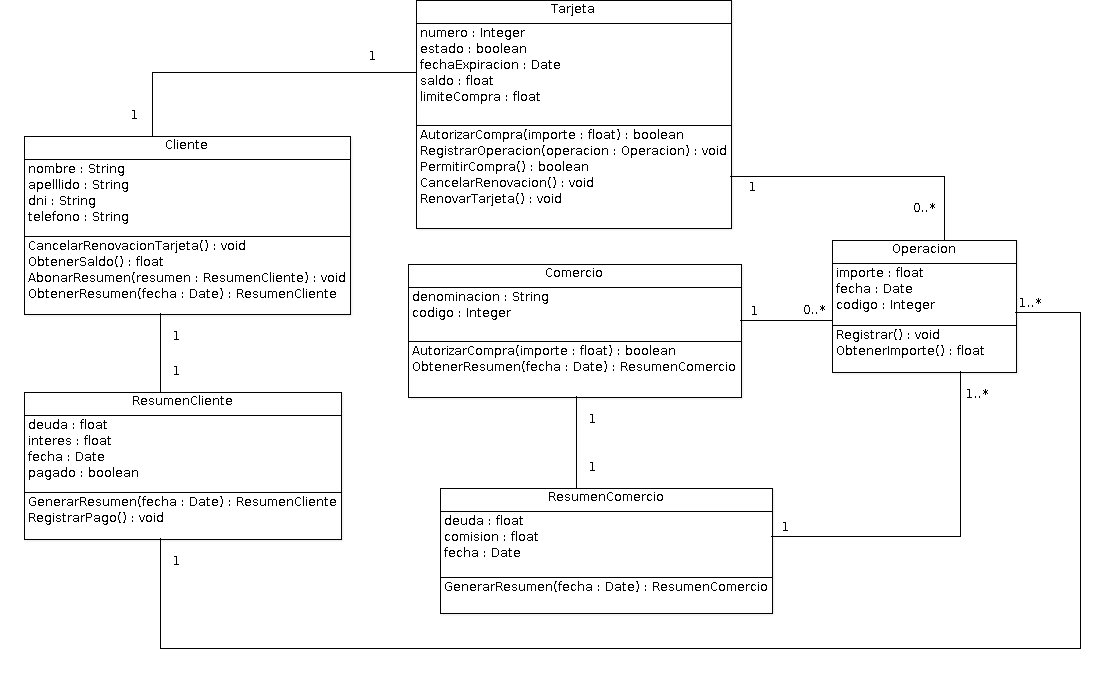
\includegraphics[width=\textwidth]{images/mod_objetos_clases.png}
\end{center}
\caption{Diagrama de clases del modelo de objetos}
\label{fig:modobjetos:diagramaclases}
\end{figure}

\FloatBarrier

En las siguientes secciones se detallarán las responsabilidades de cada una de
las clases del diagrama de la figura~\ref{fig:modobjetos:diagramaclases}.

\subsection{Cliente}

Representa una persona física que se ha registrado en el sistema y que ha
recibido una tarjeta ShoppyCard. Contiene los datos personales de dicho 
individuo.

\subsection{Tarjeta}

Representa los conceptos asociados a una tarjeta de un cliente. Contiene los 
datos asociados a la tarjeta física de la persona, como por ejemplo el número
identificatorio del plástico, pero también los datos pertinentes a la cuenta 
del cliente accesible a través de la tarjeta, como son el saldo y el límite de
compra.

\subsection{Operacion}

Representa una operación de compra que un cliente realiza en un comercio, y que
fue informada por dicho local a través del caso de uso ``Informar Ventas'' de 
la sección~\ref{sec:modcasos:informarventas}. Contiene el importe de la compra,
pero también datos de auditoría relacionados al movimiento, como la fecha en la
que fue realizado.

\subsection{Comercio}

Representa un local del shopping registrado en el sistema para permitir a sus
clientes abonar por los productos y/o servicios que vende a través de la 
tarjeta. Contiene datos de referencia relacionados al comercio.

\subsection{ResumenCliente}

Representa un resumen de cuenta de un cliente emitido en el caso de uso 
``Emitir Resúmenes''. 

\subsection{ResumenComercio}

Representa un resumen de cuenta de un comercio emitido en el caso de uso
``Emitir Resúmenes''. 

\section{Diagramas de interacción}

A modo ejemplificativo, desarrollaremos a continuación en detalle los 
diagramas de interacción relacionados con el relevamiento del caso de uso
``Informar Ventas'', detallado en la sección~\ref{sec:modcasos:informarventas}.

En la figura~\ref{fig:modobjetos:diagramasecuencia} se detalla el diagrama de 
secuencia asociado a dicho proceso. En particular, se presenta la secuencia de
mensajes asociados al procesamiento de uno de los registros de ventas que 
informa un comercio particular en dicho caso de uso.

\begin{figure}[htb]
\begin{center}
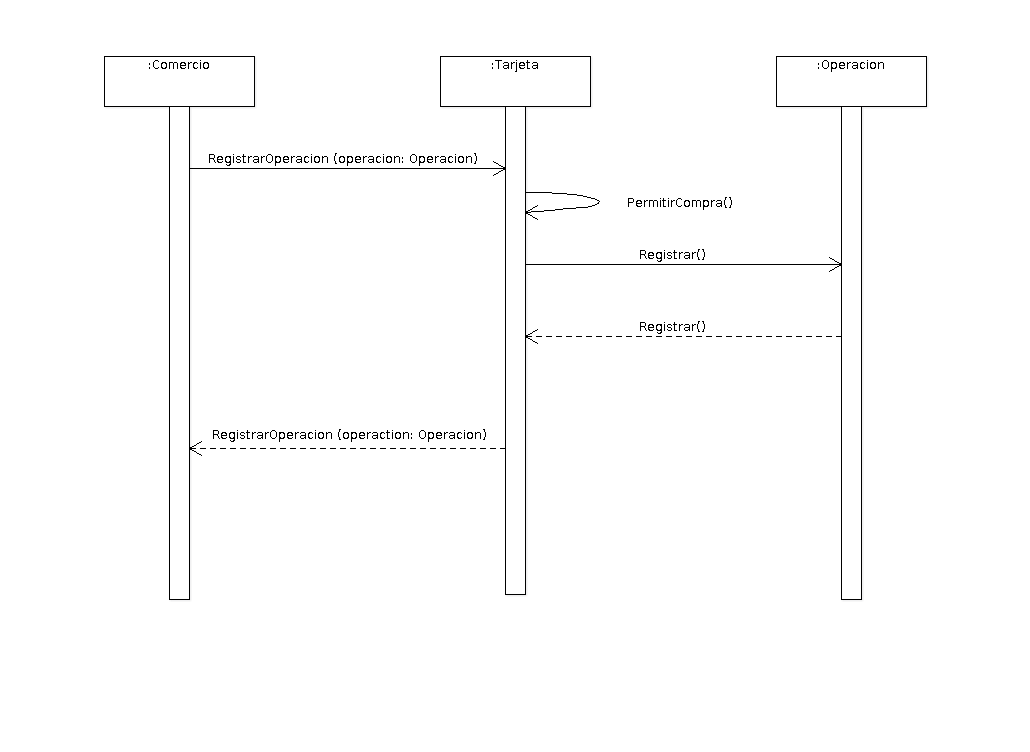
\includegraphics[width=0.9\textwidth]{images/mod_objetos_secuencia.png}
\end{center}
\caption{Diagrama de secuencia para el caso de uso Autorizar Compra}
\label{fig:modobjetos:diagramasecuencia}
\end{figure}

\FloatBarrier

En la figura~\ref{fig:modobjetos:diagramacolaboracion} se detalla el diagrama
de colaboración asociado al caso de uso analizado. Nuevamente, se detallan las
interacciones que se realizan al procesar uno de los registros de ventas que
informa un comercio particular en el caso de uso analizado.

\begin{figure}[htb]
\begin{center}
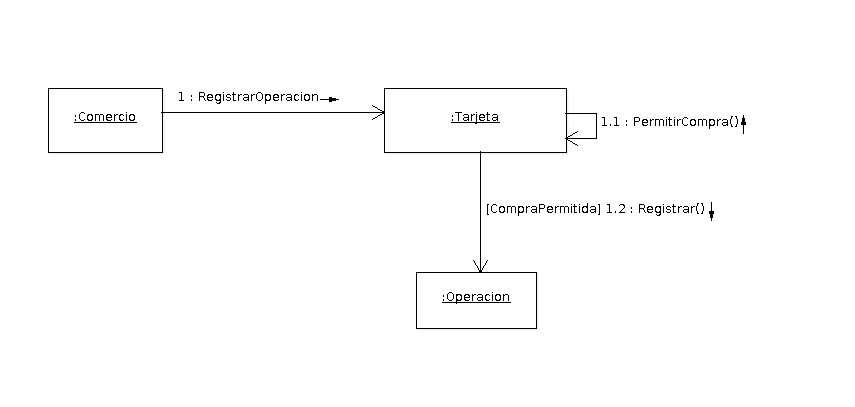
\includegraphics[width=\textwidth]{images/mod_objetos_colaboracion.png}
\end{center}
\caption{Diagrama de colaboración para el caso de uso Autorizar Compra}
\label{fig:modobjetos:diagramacolaboracion}
\end{figure}

\FloatBarrier

Ambos diagramas explican el proceso de un registro de venta informado por un comercio.
El comercio registra una operación de venta en la tarjeta. Esta valida la 
operación de acuerdo a las reglas del caso de uso (la fecha de la operación debe
corresponder al mes actual, por ejemplo). Si la compra es válida, la
operación es registrada.

\FloatBarrier
